% !TEX root = ../partial-sdm.tex

The framework has been validated comparing its results with the expected results from \citet{Kanerva1988}. Thus, we run simulations which were then compared to the theoretical analysis conducted some decades ago.

\section{Distance between random bitstrings}

As shown by \citet{Kanerva1988}, the distance between two bitstrings follows a binomial distribution with mean $\mu = n/2$ and standard deviation $\sigma = \sqrt{n}/2$. For large values of $n$, it may be approximated by a normal distribution with the same mean and standard deviation.

In order to validate our random bitstring generation algorithm, we have calculated 10,000 distances between two random bitstrings with $n=1,000$ bits. In total, 20,000 random bitstrings have been generated during the simulation. The code is available in the ``Distance between bitstrings'' notebook \citep{sdmframework}.

In figure \ref{fig:validation-distance}, we can notice that the theoretical model and the simulation matches. Hence, it seems the random bitstring generation algorithm works properly.

This also validates the algorithm used to calculate the distance between two bitstrings. In this simulation, we have used the built-in \_\_popcnt() function.

\begin{figure}[!htb]
  \centering
  \subfloat[Full histogram ]{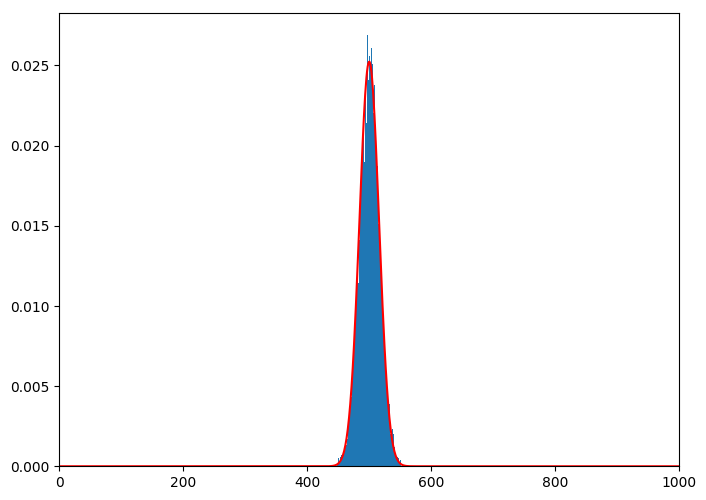
\includegraphics[width=0.5\textwidth]{./images02/new-images/bs-hist-full.png}}
  \subfloat[{Zoom in the interval $[400, 600]$} ]{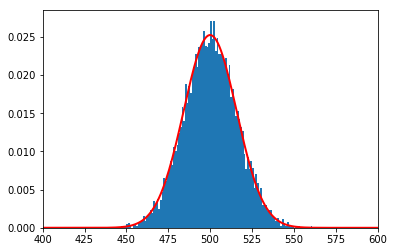
\includegraphics[width=0.5\textwidth]{./images02/new-images/bs-hist-zoom.png}}

  \caption{Histogram of 10,000 distances between two random bitstrings with 1,000 bits. The curve in red is the theoretical normal distribution with $\mu = 500$ and $\sigma = \sqrt{500}/2$.}
  \label{fig:validation-distance}
\end{figure}


\section{Number of activated hard locations}

In his seminal work, Kanerva proposed to use a sample of 1,000,000 hard locations in a 1,000 bits SDM. He also proposed to activate only 1,000 of them, on average. He calculated that an access radius of $r=451$ would activate, on average, 0.00107185004892 of the whole space, or, in this case, 1,071.85 hard locations.

We extended his results, calculating the distribution of the number of activated hard locations. As each hard location has probability $p=0.00107185004892$ of being activated, the probability of activating exactly $a$ out of $H$ hard locations follows a binomial distribution with mean $\mu = pH$ and standard deviation $\sigma = \sqrt{Hp(p-1)}$. In this case, $\mu = 1071.85$ and $\sigma = 32.72$.

In order to validate our scan algorithm, we have run 10,000 scans from a random bitstring and counted the number of activated hard locations. The code is available in the ``Number of activated hard locations'' notebook \citep{sdmframework}.

In figure \ref{fig:validation-activated-hls}, we can notice that the theoretical model and the simulation matches. Hence, it seems that both the address space generation algorithm and the scan algorithm work properly. Notice that the curve is almost the same for $n=1,000$ and $n=256$. It happens because the access radius is adjusted to get $p$ as close as possible to $0.001$. They are not exactly the same because their $p$ differs a little.

\begin{figure}[!htb]
  \centering
  \subfloat[$n=1,000$, $H=1,000,000$,\protect\\ $r=451$, and $p=0.00107185$ ]{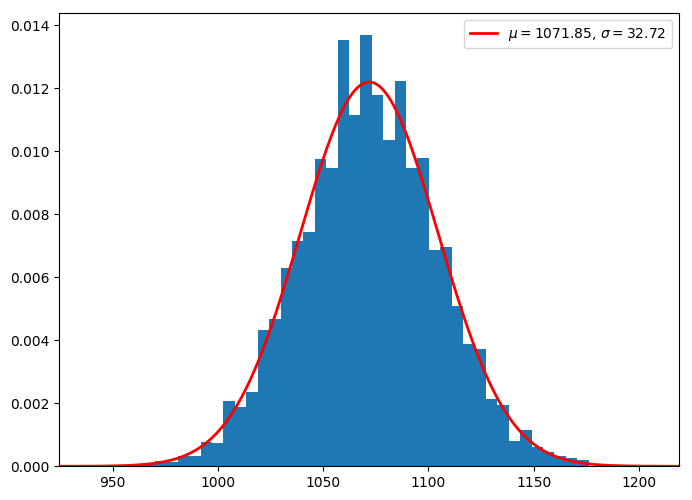
\includegraphics[width=0.5\textwidth]{./images02/new-images/activated-hls-1000.png}}
  \subfloat[$n=256$, $H=1,000,000$,\protect\\ $r=103$, and $p=0.00106684$ ]{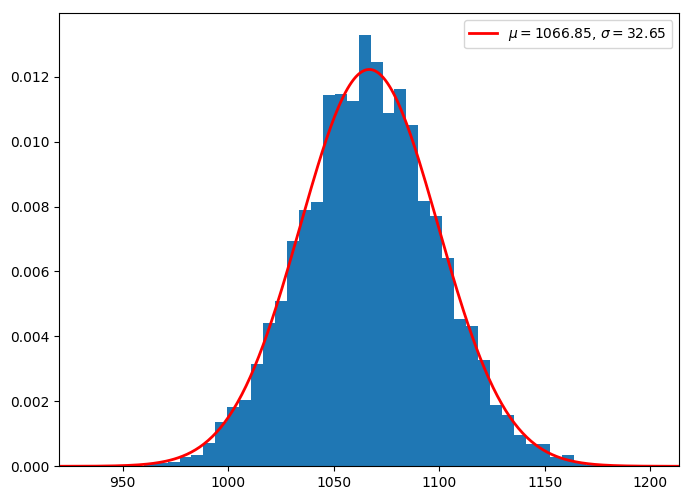
\includegraphics[width=0.5\textwidth]{./images02/new-images/activated-hls-256.png}}

  \caption{Histogram of the number of activated hard locations in 10,000 scans from a random bitstring. The curve in red is the theoretical normal distribution with $\mu = Hp$ and $\sigma = p(p-1)H$.}
  \label{fig:validation-activated-hls}
\end{figure}

Besides the number of activated hard locations, we have also extended Kanerva's results to calculate the distribution of distances between the center of the circle and the activated hard locations. Let $A$ be the set of activated hard locations, $\xi$ be the center of the circle, and $r$ be the access radius, then:

\begin{align}
P(\text{d}(a, \xi)=x | a \in A) &= \frac{P(\text{d}(a, \xi)=x)}{P(a \in A)} \\
    &= \frac{\binom{n}{x}}{\sum_{k=0}^r \binom{n}{k}} \label{eq:prob-d-inside-circle}
\end{align}

In order to check Equation \ref{eq:prob-d-inside-circle}, we have calculated the distances of the activated hard locations to the center of 1,000 random circles. The code is available in the ``Distances of activated hard locations'' notebook \citep{sdmframework}.

In figure \ref{fig:validation-distance-activated-hls}, we can notice that the theoretical model and the simulation matches.

\begin{figure}[!htb]
\centering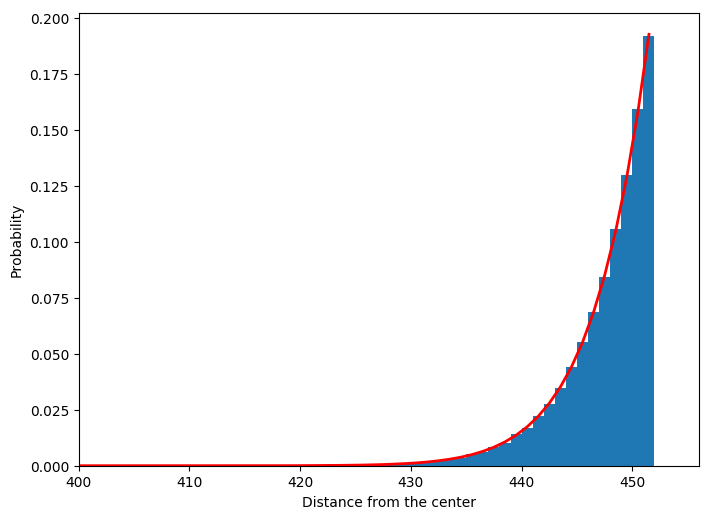
\includegraphics[width=\textwidth]{./images02/new-images/distance-activated-hls.png}

\caption{Histogram of the distances of activated hard locations to the center of the circles. The curve in red is the theoretical distribution of Equation \ref{eq:prob-d-inside-circle}
\label{fig:validation-distance-activated-hls}}
\end{figure}

\section{Intersection of two circles}

Kanerva has calculated the intersection of two circles according to the distance between their centers. The intersection is important to understand how SDM works because it affects directly the critical distance. When $\eta_d$ is inside the critical distance, then it will converge to $\eta$. In fact, it converges because they share a sufficient amount of hard locations, i.e., the intersection of the circle around $\eta_d$ and $\eta$ is enough to converge. For further information about the relation between the critical distance and the intersection, see \citet{brogliato2014sparse}.

We have calculated the intersection between a random bitstring (bs1) and another bitstring (bs2) exactly $d$ bits away. The former (bs1) is just a random bitstring. The latter (bs2) was generated randomly flipping $d$ bits of bs1. The code is available in the ``Kanerva's Figure 1.2'' notebook \citep{sdmframework}.

In Figure \ref{fig:validation-intersection}, we can notice that we have obtained the same results as Kanerva. It seems that the random flipping bits algorithm and the scan algorithm work properly.

\begin{figure}[!htb]
  \centering
  \subfloat[{\citet[Figure 1.2, p.25]{Kanerva1988}} ]{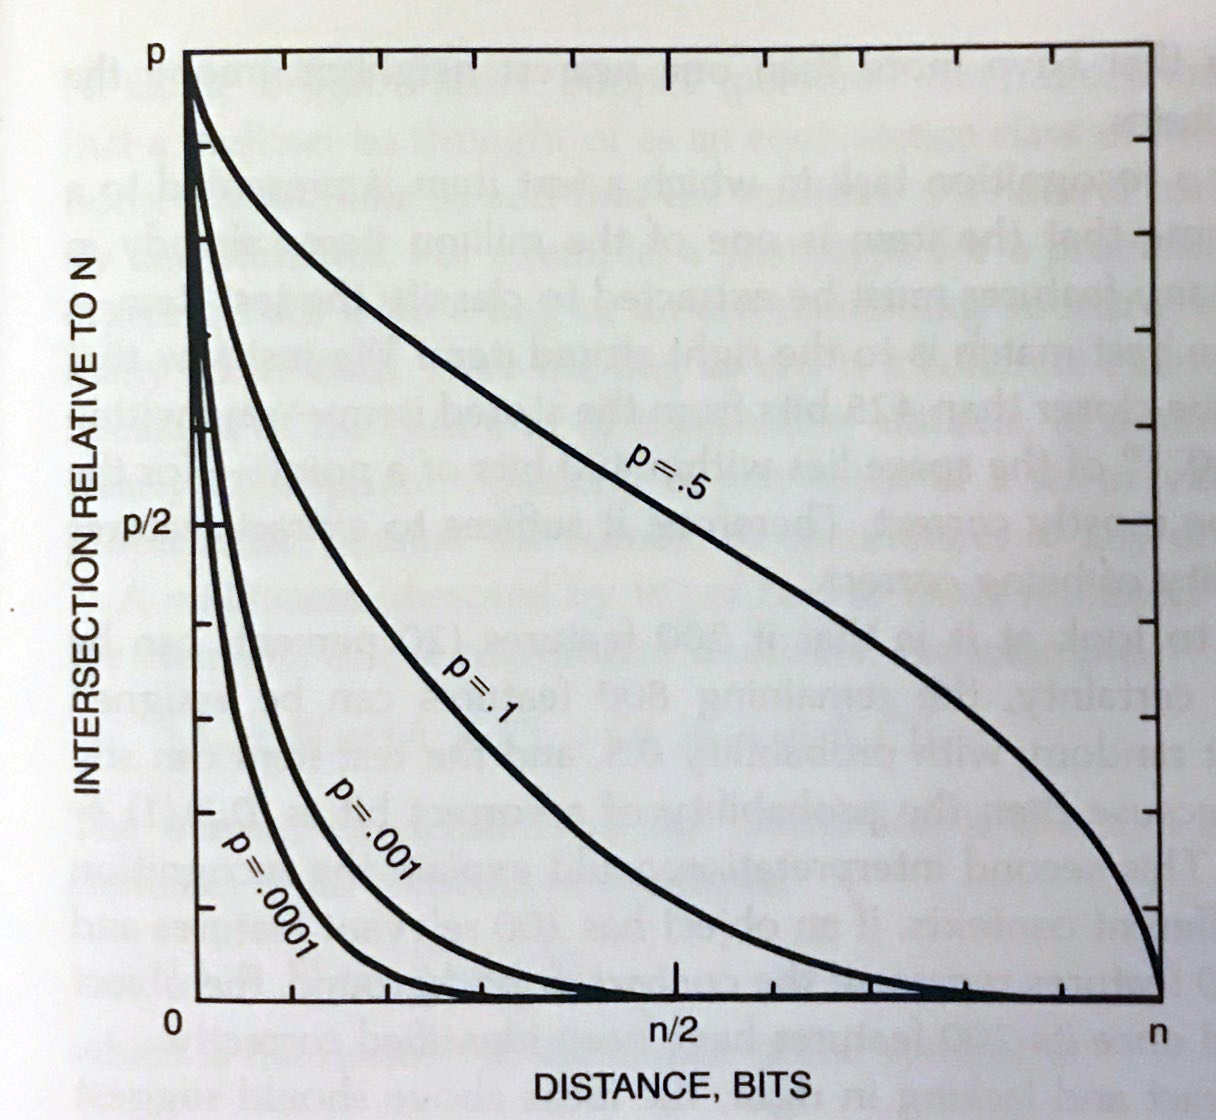
\includegraphics[width=0.45\textwidth]{./images02/new-images/kanerva-table-12.jpg}}
  \subfloat[Generated by SDM framework with $n=1,000$ ]{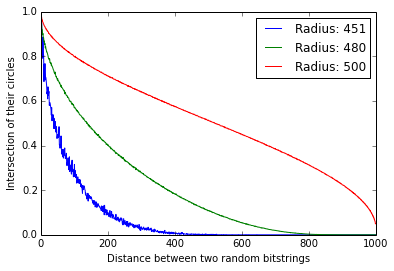
\includegraphics[width=0.55\textwidth]{./images02/new-images/intersection-of-circles.png}}

  \caption{Number of hard locations in the intersection of circles around two bitstrings $x$ bits away.}
  \label{fig:validation-intersection}
\end{figure}


\section{Storage and retrieval of sequences}

\citet[Ch.8]{Kanerva1988} presented an approach to store and retrieve sequences using $k$ different SDMs, namely $\text{sdm}_1$, $\text{sdm}_2$, $dots$, $\text{sdm}_k$.

Let $a_0, a_1, a_2, \dots, a_n$ be a sequence to be stored in a $k$-fold memory. So, all pointers of the form $a_i \rightarrow a_{i+k}$ will be written to $\text{sdm}_k$ memory, i.e., in $\text{sdm}_1$, the following pointers will be written: $a_0 \rightarrow a_1$, $a_1 \rightarrow a_2$, $\dots$, $a_{n-1} \rightarrow a_n$; while in $\text{sdm}_2$, the following pointers will be written: $a_0 \rightarrow a_2$, $a_2 \rightarrow a_3$, $\dots$, $a_{n-2} \rightarrow a_n$; and so forth.

We have tested exactly the same example presented in \citet{Kanerva1988}, p.85. We wrote two sequences to a $3$-fold memory: $<A, B, C, D>$ and $<E, B, C, F>$. Then, after reading the sequences $<A, B, C>$ and $<E, B, C>$, we have obtained $D$ and $F$, respectively.

Each reading operation was performed summing the counters of all activated hard locations from all three memories. For instance, to read the sequence $<A, B, C>$, we have activated the hard locations around $C$ in $\text{sdm}_1$, we have also activated the hard locations around $D$ in $\text{sdm}_2$, and, finally, we have also activated the hard locations around $A$ in $\text{sdm}_3$. After summing the counters of all those hard locations, we evaluate the resulting bitstring just as in the original read operation.

The code is available in the ``Sequences (Kanerva Ch 8)'' notebook \citep{sdmframework}.

The logic behind how it works is that, when reading the sequence $<A, B, C>$, we have $A$ pointing to $D$, while both $B$ and $C$ point to $D$ and $F$. Thus, $D$ appears more often than $F$ and ended up being the result.

Hence, as we have replicated the theoretical results from Kanerva, we have one more evidence that our framework works properly.

\subsection{$k$-fold memory using only one SDM}

We have extended Kanerva's ideas to be able to store and retrieve sequences in $k$-fold memories using only one SDM (instead of $k$ SDMs).

Our idea was to create $k$ random bitstrings, one for each fold. We have performed writing and reading exactly as Kanerva's original idea, but, instead of writing to $\text{sdm}_k$, we have written $a_{i+k}$ into the address $a_i \oplus \text{tag}_k$, and, instead of reading from $\text{sdm}_k$, we have read from address $a_i \oplus \text{tag}_k$, where $\oplus$ is the exclusive or (XOR) operator.

It worked as if we had split SDM into $k$ regions with low intersection between two of them. So, as the interference is minimal, they work like independent SDMs. The major disadvantage of this approach is that memory capacity may be reached faster.

Splitting the memory into regions may be an interesting strategy to other sorts of problems, mostly the ones which would need many SDMs and, consequently, would use a lot of RAM.
